\chapter{Background}

In this chapter, we will provide an introduction to the Scala programming language. 
We will showcase a running example that we will use for the remainder of this thesis which we believe exhibits features commonly present in Scala programs. 
We will describe \acrfull{tasty}, an intermediate storage format used for separate compilation\cite{???} of Scala programs. 
We will introduce a critical transformation, type erasure, which alters Scala programs so that they may executable on their default platform the \acrfull{jvm}. 
We will detail GraalVM \acrfull{jit} compiler infrastructure, an alternative JVM implementation which we use to implement a runtime for Scala in this thesis.

\section{Scala}

Scala\cite{scala:overview} is a objected-oriented, generic and statically typed programming language.
Scala uses a \textit{pure} object-oriected programming model\cite{smalltalk:design} and addresses many of the shortcomings\cite{go4:design-patterns} in other object-oriented programming languages.
Scala can be still considered \textit{Java-like} because of the interoperability between Java and Scala programs.
Programs in Scala may contain generic definitions, allowing Scala programs to composable and reusable\cite{scala:origins}.
We describe the programming paradigms present in Scala in detail:

\begin{description}
	\item[Object-oriented] 
	Every value in Scala is an object and every operation is method invocation on an object. 
	Every object in Scala is an instance of a \textit{class} and their type is determined by their class.
	Classes\cite{simula:classes} are a mechanism for defining state and behaviour for a group of objects.	
	
	\item[Generic] 
	Classes in Scala may contain \textit{type parameters} and such classes can be considered \textit{polymorphic}\cite{strachey:fundamental-concepts}.
	Polymorphic classes may define behavior independent of their state, allowing polymorphic classes to be reused extensively for multiple types of data.
	
	\item[Statically typed] 
	Static typing is a discipline where the type information about a program is known \textit{before} it is executed.
	In order for a Scala program to compile successfully, it must be \textit{well-typed}.
	Classes are the primary syntactical mechanism for declaring types in Scala. 
	The properties of classes such as state, in the form of fields, and behaviour, in the form of methods, must be well-typed.
	Similarly, the uses of these properties in other classes must also be well-typed. 
\end{description}

\section{Case Study: A List in Scala}

In this section, we will introduce the running example that will be used for the remainder of this thesis and our motivations for its selection.
Figures \ref{example:list-def}, \ref{example:cons-impl} and \ref{example:nil-impl} contain an abstract singly-linked list class and its two concrete subclass implementations. 
We believe these \scalainline{List} implementations should represent a real-world use case as they are a scaled down and simplified version of the list implementation present in the Scala collections library.
The \scalainline{List} definition from the collections library is available by default to all Scala programs.

\begin{figure}[!htb]
	\begin{minted}{scala}
	abstract class List[+T] {
		def head: T
		def tail: List[T]
		def length: Int
		def isEmpty: Boolean = length == 0
		def contains[T1 >: T](elem: T1): Boolean
	}
	\end{minted}
	\caption{Definition of \texttt{List} class}
	\label{example:list-def}
\end{figure}

Figure \ref{example:list-def} is an example which showcases the paradigms discussed in the previous section that are also commonly present real-world Scala programs.
Implementations which derive abstract the \scalainline{List} class will demonstrate \textit{class inheritance}.
The \scalainline{List} class contains both polymorphic and non-polymorphic methods to showcase type specialization.
The \scalainline{head} method is class-polymorphic in that its type is derived from a class parameter and becomes specialized when the class is specialized.
The \scalainline{contains} method is method-polymorphic and must be specialized after the class is specialized.

\begin{figure}[!htb]
	\begin{minted}{scala}
	case class Cons[+T](head: T, tail: List[T]) extends List[T] {
		override def length: Int = 1 + tail.length
		
		override def contains[T1 >: T](elem: T1): Boolean = {
			var these: List[T] = this
			while (!these.isEmpty) 
			if (these.head == elem) return true
			else these = these.tail
			false
		}
			
		override def hashCode(): Int = {
			var these: List[T] = this
			var hashCode: Int = 0
			while (!these.isEmpty) {
				val headHash = these.head.## // Compute hashcode
				if (these.tail.isEmpty) hashCode = hashCode | headHash
				else hashCode = hashCode | headHash >> 8
				these = these.tail
			}
			hashCode
		}
	}
	\end{minted}
	\caption{Implementation of \texttt{Con} class}
	\label{example:cons-impl}
\end{figure}

Figure \ref{example:cons-impl} contains the implementation of a list node.
The \scalainline{Cons} implementation contains two polymorphic fields, \scalainline{head} and \scalainline{tail}.
For specialization, we only care about \scalainline{head} as a field does not change to store a \scalainline{List[Int]} or \scalainline{List[Double]}.
On the other hand, the layout of the class would change if the head field was meant to store an integer instead of a byte.

\begin{figure}[!htb]
	\begin{minted}{scala}
	case object Nil extends List[Nothing] {
		override def head: Nothing = throw new NoSuchElementException("head of empty list")
		override def tail: Nothing = throw new UnsupportedOperationException("tail of empty list")
		override def length: Int = 0
		override def contains[T1 >: Nothing](elem: T1): Boolean = false
		override def hashCode(): Int = 0
	}
	\end{minted}
	\caption{Implementation of \texttt{Nil} class}
	\label{example:nil-impl}
\end{figure}

Figure \ref{example:nil-impl} contains the implementation of the empty list. 
We provide the implementation of this class for completeness.


\section{Typed Abstract Syntax Trees}

An \acrfull{ir} is a structural abstraction representing a program during compilation or execution. 
Intermediate representations are more suitable for reasoning about a program than program source code. 
\acrshort{ir} can be used for compilation\cite{llvm}, optimization\cite{llvm}\cite{ssa}, or execution\cite{java:vm-spec}\cite{clr:spec}.

\acrfull{tasty} is a high-level \acrfull{ir} which is produced and emitted after type checking phase of the Scala compiler (see appendix \ref{appendix:dotty-phases}).
Figure \ref{system:tasty} gives an overview of TASTy generation in the context of the Scala compilation pipeline, note that TASTy is only generated for Scala program sources.
TASTy is a well-typed variation of an \acrfull{ast}, an IR which is close to the program source representation.
TASty can be considered a \textit{complete} IR of a Scala program before compilation, unlike the other intermediate representations we will examine throughout this thesis.
A complete IR is able to capture all information of the original Scala source program, we will expand on why this is significant in section \ref{background:type-erasure}.

\begin{figure}[H]
	\centering
	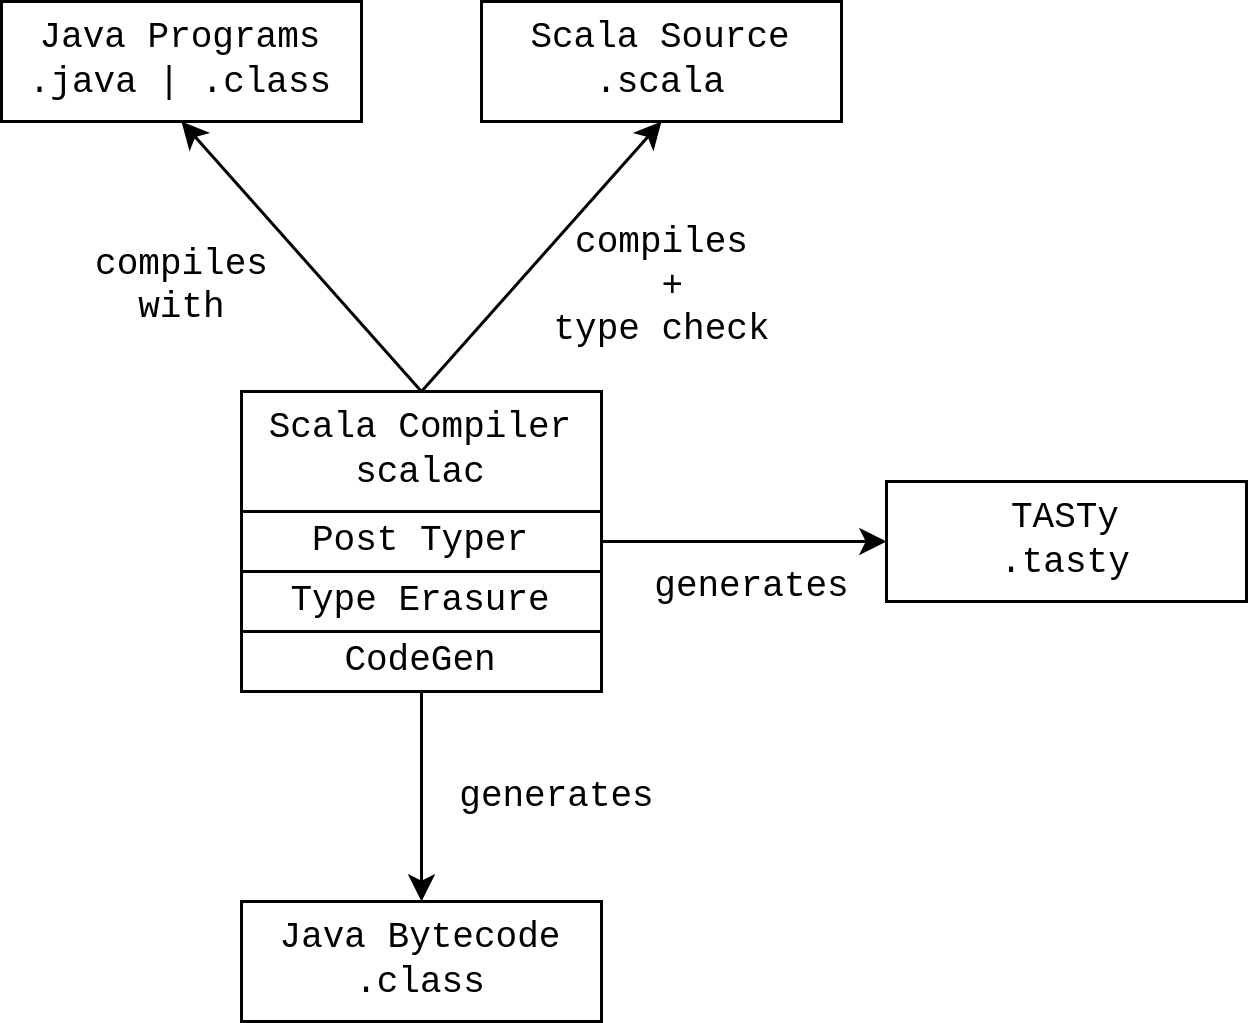
\includegraphics[width=0.5\textwidth]{figures/scala-pipeline.png}
	\caption{TASTy in the context of the Scala compilation pipeline.}
	\label{system:tasty}
\end{figure}

In this thesis, we will use a limited subset of TASTy which is sufficient to represent the program given in figures \ref{example:list-def} and \ref{example:list-impl}.
The TASTy trees used in this thesis can be divided into categories, definitions, terms, and types. 
We give the pseudo implementations of these trees in figures \ref{tasty:defs}, \ref{tasty:terms}, and \ref{tasty:types}.

\subsection{Definitions}

\begin{figure}[!htb]
	\begin{minted}{scala}
	trait Tree                         // Tree representing code written in the source
	trait Statement extends Tree       // Tree representing a statement in the source code
	trait Definition extends Statement // Tree representing a definition in the source code.
		
	// Tree representing a class definition.
	case class ClassDef(
		constructor: DefDef, 
		parents: List[Tree], 
		self: Option[ValDef], 
		body: List[Statement]
	) extends Definition
	// Tree representing a method definition in the source code
	case class DefDef(params: List[ParamClause], returnTpt: TypeTree, rhs: Option[Term]) extends Definition
	// Tree representing a value definition in the source code.
	case class ValDef(name: String, tpt: TypeTree, rhs: Option[Term]) extends Definition
	// Tree representing a type (parameter or member) definition in the source code
	case class TypeDef(name: String, rhs: Tree) extends Definition
	\end{minted} 
	\caption{Pseudocode class definitions for a subset of TASTy trees.}
	\label{tasty:defs}
\end{figure}

Figure \ref{tasty:defs} will provides the pseudo implementations of all definitions in our subset of TASTy.
Our subset of TASTY contains all definition trees from TASTy.
For most of the definitions, they can be translated and be represented by a corresponding implementation in Truffle.
A \scalainline{ClassDef} always represents a top level class definition.
A \scalainline{DefDef} tree is always the definition of a method inside a class definition.
Despite having every definition tree from regular TASTy available, we will omit the discussion of more complex definitions such as nested classes or closures.
% show grammar?s

\subsection{Terms}
\begin{figure}[!htb]
	\begin{minted}{scala}
	trait Term extends Statement       // Tree representing an expression in the source code
	trait Ref extends Term             // Tree representing a reference to definition
	
	// Tree representing an assignment lhs = rhs in the source code
	case class Assign(lhs: Term, rhs: Term) extends Term
	// Tree representing new in the source code
	case class New(tpt: TypeTree) extends Term
	// Tree representing a block `{ ... }` in the source code
	case class Block(statements: List[Statement], expr: Term) extends Term
	// Tree representing a while loop
	case class While(cond: Term, body: Term) extends Term
	// Tree representing a selection of definition with a given name on a given prefix
	case class Select(qualifier: Term, selector: String) extends Term 
	// Tree representing an application of arguments.
	case class Apply(applicator: Term, arguments: List[Term]) extends Term
	// Tree representing an application of type arguments
	case class TypeApply(fun: Term, args: List[TypeTree]) extends Term
	// Tree representing a reference to definition with a given name
	case class Ident(name: String) extends Ref 
	\end{minted} 
	\caption{Pseudocode class definitions for a subset of TASTy trees.}
	\label{tasty:terms}
\end{figure}

Figure \ref{tasty:terms} gives the implementation for terms in our subset of TASTy.
Terms represent an executable atom of code which returns a value.
Our term tree subset of TASTy represents a basic language with support for simple imperative programming with control flow constructs such as branching and loops.
A basic set of object-oriented features are also encapsulated in the tree definitions given above such as object creation, instance method invocation, and instance field access.
Our subset also supports the creation of polymorphic classes as well as the invocation of polymorphic methods.

\subsection{Type Trees}
\begin{figure}[!htb]
	\begin{minted}{scala}
	// Type tree representing a type written in the source
	trait TypeTree extends Tree 
	
	// Type tree representing a reference to definition with a given name
	case class TypeIdent(name: String) extends TypeTree 
	// Type tree representing a type application
	case class Applied(tpt: TypeTree, args: List[TypeTree | TypeBoundsTree]) extends TypeTree
	// Type tree representing a type bound written in the source
	case class TypeBoundsTree(lo: TypeTree, hi: TypeTree) extends TypeTree
	\end{minted} 
	\caption{Pseudocode class definitions for a subset of TASTy type trees.}
	\label{tasty:types}
\end{figure}

Type trees are a subset of trees which represent types as they are declared in Scala source code.
Figure \ref{tasty:types} gives the subset of type trees which we will use in this thesis.
For our purposes, there are only three ways to refer to types.
A \scalainline{TypeIdent} type tree is a reference to a type which is monomorphic \scalainline{ClassDef}.
An \scalainline{Applied} type tree represents a type constructor, which accept type arguments and produce a new type.
For example, the \scalainline{Cons[T]} would be represented as an applied type tree, where \scalainline{Cons} would the constructor and \scalainline{T} would be the type argument.
A \scalainline{TypeBounds} tree represents the type expression \scalainline{Lo <: T <: Hi}, a constraint where \scalainline{T} must be a subtype of type \scalainline{Hi} and supertype of type \scalainline{Lo}.
In the context of this thesis, we can use subtype to mean \textit{subclass of} and supertype of \textit{superclass of}.

We will go over each tree and their relevance for execution in our interpeter in chapter \ref{chapter:implementation}.
As part of normal Scala compilation pipeline, TASTy is eventually transformed by the Scala compiler and converted into Java bytecode. 
In the next section, we detail a critical compilation phase which enables the Scala compiler generate correct Java bytecode.

\section{Type Erasure}
\label{background:type-erasure}

Type erasure\cite{java:generics} is a transformation which converts polymorphic classes methods in Scala to monomorphic classes and methods. 
This conversion is necessary because the JVM does not support polymorphic classes during runtime.
Erasure ensures that any given polymorphic class and method has a single representation in practice.
Type erasure is a crucial part of the Scala compilation which renders TASTy incomplete.
Figure \ref{example:erase-cons} shows the \scalainline{Cons} class after type erasure.

\begin{figure}[!htb]
	\begin{minted}{scala}
	case class Cons(head: Any, tail: List) extends List {
		override def length: Int = 1 + tail.length
			
		override def contains(elem: Any): Boolean = {
			var these: List = this
			while (!these.isEmpty) 
			if (these.head == elem) return true
			else these = these.tail
			false
		}
			
		override def hashCode(): Int = {
			var these: List = this
			var hashCode: Int = 0
			while (!these.isEmpty) {
				val headHash = these.head.##
				if (these.tail.isEmpty) hashCode = hashCode | headHash
				else hashCode = hashCode | headHash >> 8
				these = these.tail	
			}
			hashCode
		}
	}		
	\end{minted}
	\caption{\scalainline{Cons} class after type erasure}
	\label{example:erase-cons}
\end{figure}

The polymorphic \scalainline{Cons} class has all type parameters in its class definition \textit{erased} and replaced by the \scalainline{Any} type.
The \scalainline{Any} type is a Scala platform-independent\cite{scala:overview} abstract type representing the super type of primitive and reference types.
In Java bytecode, the {Any} type resolves to the \scalainline{Object} type, the super type of all reference types on the JVM.

While type erasure simplifies classes for runtime, the Scala compiler must resolve the incompatibility of operations between primitives types and reference types on the JVM\cite{java:vm-spec},
The set of operations introduced by the compiler whenever a primitive value is accessed under a polymorphic context is known as \textit{autoboxing}\cite{java:autoboxing}. 
Autoboxing can be divided into two operations.
\textit{Boxing} occurs when a primitive value must be used where a generic value is expected.
\textit{Unboxing} occurs when a generic value must be used where a primitive value is expected.
Figure \ref{example:autoboxing} shows a simple example of inserted autoboxing operations when using the polymorphic \scalainline{Cons} class after type erasure.

\begin{figure}[!htb]
	\begin{minted}{scala}
	// Before type erasure 	
	val lst: List[Int] = Cons(1, Nil)
	val head: Int = lst.head
	// After type erasure
	val lst: List = Cons(box(1), Nil)
	val head: Int = unbox(lst.head) 
	\end{minted}
	\caption{Example of autoboxing introduced for a list}
	\label{example:autoboxing}
\end{figure}

The \scalainline{head0} field inside the \scalainline{Cons} class after erasure is no longer polymorphic and instead has the type \scalainline{Any}. 
The integer value of \scalainline{1} which is passed into the class constructor for the list is boxed and the primitive value is wrapped as a instance of its boxed class.
Similarly, when the \scalainline{head0} field of the instance is read and stored into a local variable, an unboxing operation occurs which extracts the primitive value out of its wrapper instance.
In the Scala collections library, a set of commonly used polymorphic data structures, autoboxing operations are frequent and necessary.
The computational overheads of autoboxing operations on programs which make substantial use of polymorphic collections, especially the Scala standard library, is significant\cite{scala:collections-optimization}.
The elimination of this overhead through optimizing autoboxing operations is one of the central goals of this thesis.

\section{Java Bytecode}

Java bytecode is a portable and compact intermediate language and instruction set used by the Java Virtual Machine to execute programs.
Traditionally, the JVM is responsible for much of the performance optimizations of Java program\cite{java:hotspot} through \acrfull{jit} compilation.
JIT compilation is an adaptive optimization which occurs after a program has begun execution.
JIT compilation is concerned with optimizing and eliminating \textit{hotspots} or portions of the program which are the slowest.


Many different JIT compilers\cite{java:sablevm}\cite{java:jikesrvm} employ \textit{speculative} techniques to transform the program under optimization.
Speculative optimizations use information collected during program execution, otherwise known as \textit{profiling}. 
Assumptions are then made about gathered profiling data in order to generate high-performance native machine code.


After most of Scala's language constructs are eliminated from programs by the compiler, Java bytecode of the program is emitted.
The resulting Java bytecode is considered an \textit{incomplete} IR of Scala source programs, as the type information found in the program source or generated during compilation is no longer present.
This becomes a particular drawback for executing Scala programs on the JVM because speculative optimizations are unable to incorporate source level semantics.

\section{GraalVM}

GraalVM\cite{java:graalvm} is an implementation of a JVM.
While other implementations of Java virtuals machines were designed specifically for Java, GraalVM was designed from the onset to be \textit{language-independent}.
GraalVM can be divided into two components. 
The first is \textit{Truffle}, a framework for translating the semantics of a source language, also called a \textit{guest language}, to take advantage of the Graal infrastrucure.
The second is \textit{Graal}, a language-agnostic JIT compilation infrastructure which handles speculative optimizations and generation of high-performance machine code.

\begin{figure}[!htb]
	\centering
	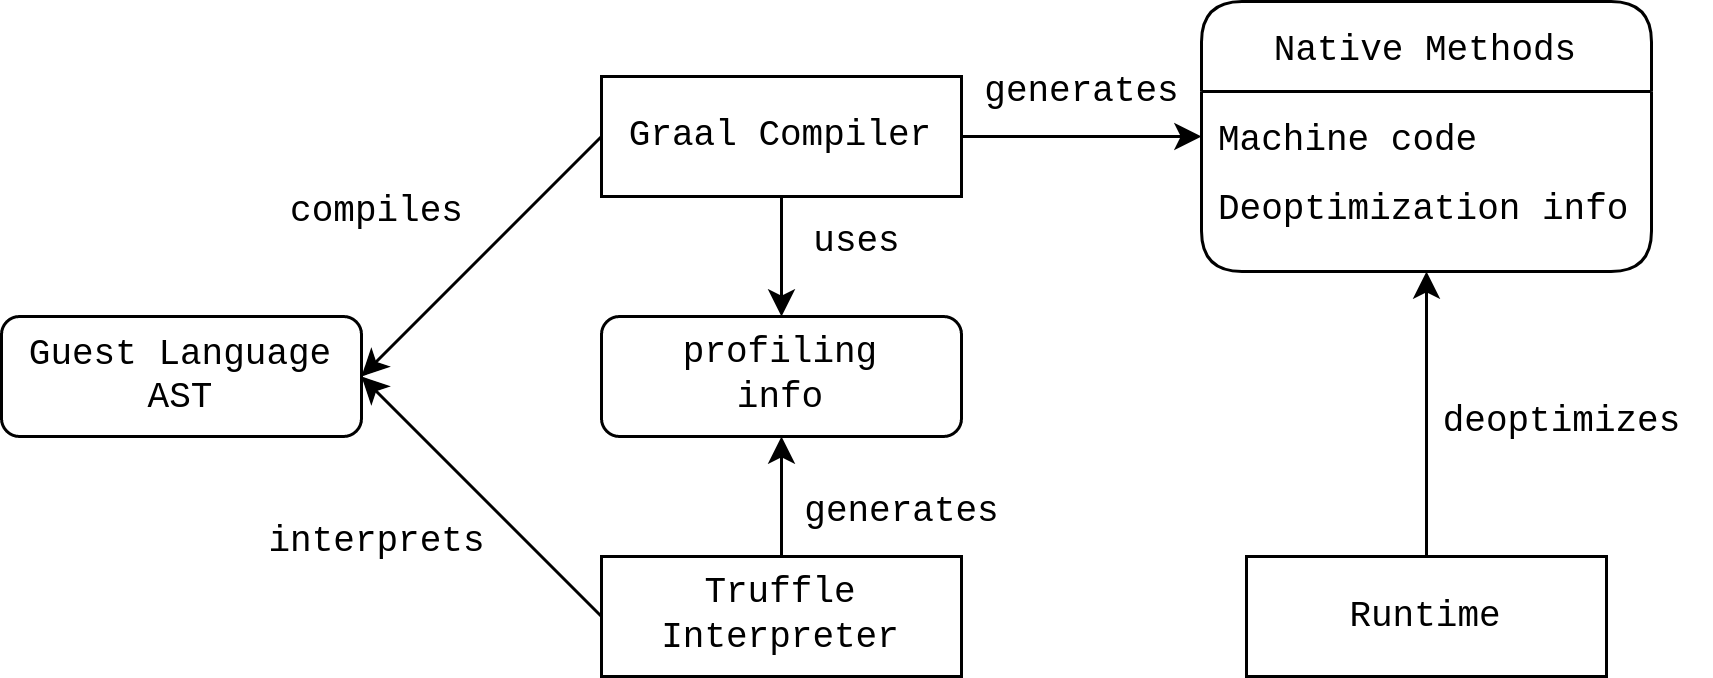
\includegraphics[width=0.7\textwidth]{figures/graalvm-pipeline.png}
	\caption{GraalVM overview\cite{graalvm:ir}.}
\end{figure}

This thesis makes substantial of both components of GraalVM to create a runtime for Scala programs using TASTy.
The runtime is able to incorporate source level information for speculative optimizations.

\subsection{Truffle}

Truffle is a \acrfull{dsl} framework for guest language implementation.
A guest language is a language which is expected to run on Graal and requires an implementation in the \textit{host language}, which provides the Truffle DSL.
In this thesis, the guest language is TASTy (which represents Scala) and the host language is Java, the implementation language of Truffle.
A guest language implementation always takes the form of an executable Truffle AST.


During execution of the AST, profiling information collected from the interpreter is used to drive \textit{node rewriting}.
While Graal is language-agnostic, Truffle is able exploit guest language semantics for dynamic optimizations.
This process of replacing nodes in the AST with better, specialized guest language counterparts in Truffle is called node rewriting.
Node rewriting serves two purposes.
The first is to dynamically incorporate guest language semantics into the executing program.
The second is to augment the AST for JIT compilation. 
In this thesis, we will focus heavily on node rewriting the execution of TASTy trees in a Truffle interpreter to augment JIT compilation.

\smartdiagramset{
	text width=2.75cm,
	uniform color list=white for 3 items,
	uniform arrow color=true,
	arrow color=black,
}
\begin{figure}[!htb]
	\centering
	\smartdiagram[circular diagram:clockwise]{
		Node rewriting,
		Partial evaluation,
		Deoptimization
	}
	\caption{Adaptive optimization loop of GraalVM}
\end{figure}

\subsection{Graal}

After node rewriting, Graal JIT compiles Truffle ASTs into native machine code using \textit{partial evaluation}.
Partial evaluation is a program optimization technique for specializing an interpreter for a given program\cite{futamura:partial-eval}.
When a Truffle AST is submitted for compilation to Graal, it is considered \textit{stable}.
This AST, previously considered an input fed into the interpreter for execution, can now be considered static data in the interpreter.
We can say that the partial evaluation of our interpreter with a given AST will produce an interpreter that can only execute the AST.

After partial evaluation, a Truffle AST is simplified to \textit{Graal IR}\cite{graalvm:ir}\footnote{Given the number of intermediate representations introduced thus far, we promise this is the last one}.
Graal IR is an IR which is suitable for speculative optimizations while still retaining information from the Truffle guest language AST.
Graal IR is based on the \textit{sea of nodes} concept\cite{click:sea-of-nodes} and sastifies the \textit{static single-assignment}\cite{ssa} property.
A sea of nodes is an abstraction based on a directed graph structure which relate the control flow graph\cite{allen:ctrl-flow-analysis} of the program to its data flow graph\cite{allen:data-flow-analysis}.
An intermediate representation is in single-static assignment form when each variable is declared once and every use of a variable occurs immediately after its declaration\cite{johnson:use-def-chains}.


GraalIR enables Graal to speculatively compile only the \textit{hot} branches\cite{graalvm:speculative-ir}, or branches that are most frequently taken, in the control flow portion of the IR and their transitive data dependencies.
When a compiled program enters an unexpected state, execution is \textit{deoptimized} and control of the program is transferred back to the interpreter.
Deoptimization occurs when the compiled program is no longer considered stable and therefore is invalid.
Graal automatically inserts \textit{guard nodes} into the IR, which are conditional checks which validate that speculative assumptions used to compile the program still hold.
Deoptimization is part of an execution loop between Graal and Truffle which allows GraalVM to aggressively adapt and speculate to find the best optimization in a dynamic environment.


